\section{Vectors and Matrices}
This section deals with operations on vectors and matrices that are commonly used.
\subsection{Vector Operations}
	\textbf{Magnitude}
	\begin{equation}
	\left\|   \vec{V} \right\|  = \sqrt{\sum_{i=1}^{n} v_i^2}
	\end{equation}
	\textbf{Dot Product}
	\begin{equation}
	\vec{V} \cdot \vec{U} = \sum_{i=1}^{n} v_iu_i
	\end{equation}
	\textbf{3x3 Cross Product}
\begin{equation}
	\vec{V} \times \vec{U} = \begin{bmatrix}
		v_2u_3 - v_3u_2\\ 
		v_3u_1 - v_1u_3\\ 
		v_1u_2 - v_2u_1
	\end{bmatrix}
\end{equation}
	\textbf{Equations with angles}
		\begin{equation}
		\cos{\theta} = \frac{\vec{V} \cdot \vec{U}}{\left\| \vec{V} \right\| \left\| \vec{U} \right\| }
		\end{equation}
		\begin{equation}
		\sin{\theta} = \frac{\vec{V} \times \vec{U}}{\left\| \vec{V} \right\| \left\| \vec{U} \right\| }
		\end{equation}
\subsection{Matrix Operations}
\textbf{Multiply}
\begin{equation}
a \times b = \begin{bmatrix}
(a_{1,1} * b_{1,1} + a_{1,2}*b_{2,1} + ...) & (a_{1,1} * b_{1,2} + a_{1,2}*b_{2,2} + ...) \\
(a_{2,1} * b_{1,1} + a_{2,2}*b_{2,1} + ...) & (a_{2,1} * b_{1,2} + a_{2,2}*b_{2,2} + ...) \\
... & ...
\end{bmatrix}
\end{equation}
\textbf{2x2 Determinant}
\begin{equation}
	det (\begin{bmatrix}
	a & b \\ c & d
	\end{bmatrix})  = ad - bc
\end{equation}
\textbf{3x3 Determinant}
\begin{equation}
	det (\begin{bmatrix}
		a & b & c\\ d & e & f \\ g & h & i
	\end{bmatrix})  = a \times det(\begin{bmatrix}
	e & f \\ h & i
	\end{bmatrix}) - b \times det(\begin{bmatrix}
	d & f \\ g & i
	\end{bmatrix}) + c \times det(\begin{bmatrix}
	d & e \\ g & h
	\end{bmatrix})
\end{equation}

\section{Fields}
This section deals with the little we need to know about Galois Fields, primarily GF(2).
\subsection{Notes}
\paragraph{Definition} Fields can be thought of as a "number system" in mathematics that has the ability to do, at least, be added and multiplied. The number system can be defined however we like, but it needs to follow a set of rules.
\begin{itemize}
	\item There must be a definition for "0" and "1" such that $x+0 = x$ and $x^*1 = 1$
	\item Addition and Multiplication are associative and commutative
	\item Multiplication distributes over addition
	\item There must be valid solutions/proofs for $a + x = 0$ and $a^*x = 1$
\end{itemize}
\paragraph{GF(2)} One particular field we use a lot is GF(2). the binary field. GF(2) only has the values "0" and "1" in its field. Multiplying in this field is the same in the field of integers we are used to, but there is one change in addition. $1 + 1$ evaluates to $0$ in GF(2).
\paragraph{Proving Laws} Prove that $a + x = 0$ and $a^*x = 1$ only have \textbf{one} solution.
\begin{equation}
\begin{split}
	x_1&= x_1 + 0 \\
	&= x_1 + (a + x_2) \\
	&= (x_1 + a) + x_2 \\
	&= (0) + x_2 \\
	&= x_2 
\end{split}
\end{equation}
\begin{equation}
	\begin{split}
	x_1&= x_1^*1 \\
	&= x_1^*(a^*x_2) \\
	&= (a^*x_1)^*x_2 \\
	&= (1)^*x_2 \\
	&= x_2 
	\end{split}
\end{equation}

\section{Lines and Planes}
This section covers everything done regarding systems of equations regarding lines and planes.
\subsection{Gaussian Elimination}
\paragraph{Algorithm} Gaussian Elimination can be described as a recursive algorithm used to solve a system of linear equations. It's a process we can use that is fairly robust. Gaussian elimination converts the system into matrix form, and we then perform row operations on it. Take for example this system.
\begin{equation}
\begin{split}
x_1 + 5x_2 - 2x_3 = -11 \\
3x_1 - 2x_2 + 7x_3 = 5 \\
-2x_1 - x_2 - x_3 = 0
\end{split}
\end{equation}
If we were to translate this to matrix form, it would look like this:

\[ \left[ \begin{array}{ccc|c}
1& 5&-2& -11 \\
3&-2& 7& 5 \\
-2&-1&-1& 0
\end{array}\right]\]

\paragraph{Row Operations} In matrix form, we can now commit to row operations. There are three possible row operations that we can use and mix and match.
\begin{itemize}
	\item Swap rows: Swap the location of two rows. (eg. R1 $\leftrightarrow$ R3)
	\item Multiply a row with a constant: You can multiply each term in a row with a constant
	\item Add two rows: You can add two rows and replace one of the addends with the sum.
\end{itemize}
Our goal with row operations to reach row echelon form; such as this form: 
\[ \left[ \begin{array}{ccc|c}
1 & 0 & 0 & a \\
0 & 1 & 0 & b \\
0 & 0 & 1 & c
\end{array}\right]\]
This is interpreted as $x_1 = a$, $x_2 = b$, and so forth.

\paragraph{Special Cases} There are two special cases
\begin{enumerate}
	\item Contradictory equations. If an equation results in a contradiction (eg. $ 0 + 0 = 1$) then we can determine that there is no solution to our system.
	\item Irrelevant equation. If one the equations becomes entirely made of $0$, then that equation is irrelevant and we have one less equation to work with. This usually results in one unknown that is then declared to be chosen freely. This can also happen when we have two equations for one unknown. 
\end{enumerate}
\paragraph{Matrix Inverse} The gaussian can also be interpreted in the form \[\mathbf{A}x = \mathbf{C}\] Where \textbf{A} is the $N \times N$ constants applied to the unknowns, \textbf{x} is the $N \times 1$ unknowns, and \textbf{C} is the $N \times 1$ constants in the equation. To solve an equation set up this way, we would normally divide A from both sides, but with matrices division isn't defined. So we need to do accomplish the inverse of multiplication another way. We do this using inverse matrices, $\mathbf{A^{-1}}$.
\newline
The inverse is defined with the following equation; \[ \mathbf{A}\mathbf{A^{-1}} = \mathbf{I}\] Where I is the identity matrix. There a few rules regarding inverse matrices that the base matrix has to pass. 
\begin{itemize}
	\item It must be a square matrix.
	\item The determinant of the matrix cannot be 0.
\end{itemize}
Once we know our base matrix has an inverse, we can find it using row operations. We do row operations on our base matrix until it reaches row echelon form. While doing so, we apply the same operations to the identity matrix. The result of the operations done on the identity matrix is the inverse matrix.
\subsection{Lines}
\paragraph{Parametric Representation} Lines, we know 'em, we love 'em. Lines are comprised of many points on a grid, and a point is comprised of coordinates. These coordinates are often represented as vectors. We are used to the normal form of a line equation; \[ y = m \times x + b\] but we have also learned how to represent a line in vector form. Given two points, $P_1$ and $P_2$, we can construct an equation.  We need to find the vector between $P_1$ and $P_2$; the difference (as $\vec{V}$) which can be interpreted as the slope. We can then take one of the points, and add it with our difference vector $\vec{V}$ multiplied with a scaling factor, and we can, using the scaling factor, generate any point on the line. \[ \mathbf{X} = P_1 + Vt\]
\paragraph{Intersecting Lines} What if we want to find the point two lines intersect? This is really easy! What we do is we set the lines equal to each other $X = Y$, and this generates a system of linear equations of sorts(where each row in the vector is an equation). Move the numbers around, and we can then use Gaussian elimination to solve for the value scaling factors. To get the point, simply plug in the appropriate scaling factor back to its parent parametric equation and the result is your point of interest.

\paragraph{Normal Form} To convert a line back to its normal form, we need to find the (unsurprisingly) normal. The normal is a $2 \times 1$ vector for lines, and can found with the following methods. Given $X = P + Vt$, $P = \begin{bmatrix}
a \\ b
\end{bmatrix}$ and $V = \begin{bmatrix}
c \\ d
\end{bmatrix}$, then the normal $N = \begin{bmatrix}
n_1 = d \\ n_2 = -c
\end{bmatrix}$ from here on, you plug in the values into the equation \[n_1x_1 + n_2x_2 = d\] all that's left is to solve for "d". in this case, $d = ad - cd$. (The d is the determinant!).

\subsection{Planes}
\paragraph{Parametric Representation} Lines are two dimensional. What if we wanted three dimensional parametric equations? These 3D sheets are called planes, and are mathematically similar to lines. Instead of being represented by two points, they are represented by three points. Given three points, $P$, $Q$ and $R$, and two scaling factors $s$ and $t$, the equation for a plane is represented by \[X = P + s \cdot \overrightarrow{PQ} + t \cdot \overrightarrow{PR}\] It's similar to that of a 2D line, just with an extra scaling factor. Solving for intersecting planes works the same way as for lines, set them equal to each other and do Gaussian Elimination.
\paragraph{Normal Form} Converting a plane to normal form is also similar to that of a line. Given the scaleable vectors $\vec{v}$ and $\vec{w}$, we can find the normal $\vec{n}$ of the plane by taking the cross product, $\vec{v} \times \vec{w}$. Given $X = P + Vt + Ws$, we find the normal as \[n_1x_1 + n_2x_2 = N \cdot P\]
\paragraph{Mirroring a Point} Sometimes, we want to mirror points on one side of a plane to the opposite side. Thinking of this theoretically, we want to find the smallest distance vector between our point $Q$ and our plane $X$, and move the point that distance on the opposite side. We need to first find the smallest distance from the plane to point. This can be done with the following formula. \[\mathbf{dist_Q} = \frac{d - (\vec{n} \cdot Q)}{\left\|\vec{n}\right\|} \cdot n\] Where 
\begin{itemize}
	\item $d$ is the constant in the normal form of the plane
	\item $\vec{n}$ is the normal of the plane
	\item $\vec{Q}$ is the point of interest
\end{itemize}
This will spit out a vector. Now, we can use this distance to find the $Q'$ point on the plane closest to the point of interest, and from there find the $Q''$ point that is the reflection of our point of interest.
\begin{equation}
\begin{split}
\vec{Q'} & = \vec{Q} + \mathbf{dist_Q} \\
\vec{Q''} & = \vec{Q} + 2 \times \mathbf{dist_Q} \\
& = \vec{Q'} + \mathbf{dist_Q}
\end{split}
\end{equation}
We can also reflect lines fairly simply. All we need to do is find the reflection of two points on the line and generate a new line from the new points. Simple and nice.
\subsection{Basis and Orthogonality}
\paragraph{Orthogonality} Vectors can have a property referred to as orthogonality. Vectors that are orthogonal are vectors that are at right angles to each other. For example, the vectors represent the x-axis and y-axis in Euclidean space are orthogonal. To test orthogonality of vectors, we just take the dot product $\vec{v} \cdot \vec{u}$ of the two vectors. If the dot product is "0", then the vectors are orthogonal. Furthermore, we can test orthogonality of lines and planes. We do this by obtaining their normals, and doing orthogonality checks on the normal vectors.
\paragraph{Vector Space} Vector space can be thought of as the number of dimensions over a certain scalar field. For example, $GF(2)^{3}$ is the 3-dimensional vector space over GF(2). Movements across n-dimensions are movements in the vector space. There is also the notion of vector sub-spaces. These are spaces of the form $s \cdot \vec{v}$, which in our work so far, are lines in 2D and planes in 3D. The equation for a line/plane is the subspace of 2D/3D vector space.
\paragraph{Linear Independence} We know how to generate subspace as lines and planes, referred to as generators. If we have generators that all point to different points in our subspace, then that's all good. But what happens if we have two generators that are scalar multiples of each other? Then we have redundant, or linearly dependent, generators. We want to be remove all redundant generators and bring our world back down to linearly independent generators. A set of linearly independent generators is referred to as a \textbf{basis}, and the number of elements in each generator is the \textbf{dimension} of the subspace. \newline
We can check linear independence using, you guessed it, Gaussian Elimination. We place all our vectors together and reduce them all to row-echelon form. Any redundant vectors will end up with all 0's in its respective row. If we have a row-echelon matrix with no special cases, then we have linear independence.

\section{Set Theory}
This section covers the basics of Set Theory, with some examples.
\subsection{Notation}
\paragraph{Set} A set is a collection of things. These things are called elements or members, and they follow the following ideas:
\begin{enumerate}
	\item Each member must be identifiable and distinguishable (aka unique)
	\item There is clear criterion defined as to whether an element is part of a set
	\item A member if a set is only counter once
	\item There is no order in a set
	\item Sets are only defined by its members. If two different sets have the same elements, as far as math if concerned, they are the same set.
\end{enumerate}

\paragraph{Set Notation} To indicate if a member $x$ is a part of a set $A$, we use the following notation. \[ x \in A\] Small, finite sets can be defined by listing out all its members; $\{Summer, Winter, Spring, Fall\}$, while infinite sets usually have a clear pattern; $\mathbb{N} = \{0, 1, 2, 3, ...\}$ We can also define subsets. A subset is a set whose elements are selected from another set. If we see $B$ as a subset of $A$, we note it as $B \subseteq A$. If we want to define $B$ with a condition, we do it as such: \[ B = \{ x \in A | x \text{ satisfies condition } c\}\] We can user formal logic, such as "there exists $\exists$" to help us define some conditions, as they can get pretty wild. Note: We can also have an empty set; an empty set is noted as $\emptyset$.
\paragraph{Set Operations} We can also do operations between sets. These are fairly simple to understand. Assume we have sets $A \subseteq X$ and $B \subseteq X$. 
\begin{enumerate}
	\item Union - $A \cup B$: Returns the set whose members are in $A$ OR $B$
	\item Intersection - $A \cap B$: Returns the set whose members are in both $A$ AND $B$
	\item Complement - $\bar{A}$: Returns the set whose members are NOT in $A$.
	\item Difference - $A \setminus B$: Returns the set whose members are IN $A$ and NOT IN $B$
\end{enumerate}
You can mix and match operations and create new ones, like the difference operation. It is equivalent to the operations $B \cap \bar{B}$.

\subsection{Cardinality} 
\paragraph{Cardinality} The cardinality of a set can be defined as the size, or amount of members in the set. The set of seasons has a cardinality of 4, for example. Sounds simple, but when we talk about the cardinality of infinite sets it is harder to give a solid number. Ofcourse, you could say they have a cardinality of "infinite", but ya boi Georg Candor discovered not all infinite sets have the same cardinality. There are two types of infinite cardinalities we concern ourselves with; countable and uncountable.
\paragraph{Countable Sets} $\mathbb{N}$ is the set of natural numbers from 0 to infinite and beyond. It is important to us because the definition of a countable set is one that has the same cardinality as the set $\mathbb{N}$. We do this by creating a sort of mapping between the set of natural numbers and whatever infinite set we are comparing. This can be seen for the set of integers $\mathbb{Z}$, by mapping each numbers negative then positive to the next position in the natural numbers, you can create a clear mapping between the two. How you create this mapping is dependent on the set you are trying to solve the cardinality for. For example, for the set of squared natural numbers $\mathbb{N^2}$, it maps in a breadth-first search style, as seen in the figure, since two natural numbers can be converted into a tuple.

\paragraph{Uncountable Set} Not all sets can be proved to be countable. A very commonly used set that is uncountable is the set of real numbers. Disproving the countability of a set is also dependent on the set you are trying to prove, but usually you want to find a mapping between each member of the natural numbers and prove that there is no such mapping. For example, in the real numbers, the values post-decimal are infinite, and each position post-decimal can be matched to a member in $\mathbb{N}$, but there are infinite number of such mappings. This means that the overall set of real numbers is uncountable. This is important to know when discussing the computability of programs, such as knowing that, because there are countabely many Java programs but uncountably many real numbers, there are some real numbers we cannot compute.
\begin{figure}[!htb]
	\center{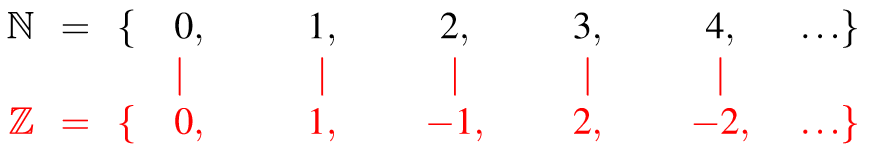
\includegraphics[width=8cm]
		{maths/countable}}
	\caption{\label{fig:zcount} N and Z}
\end{figure}
\begin{figure}[!htb]
	\center{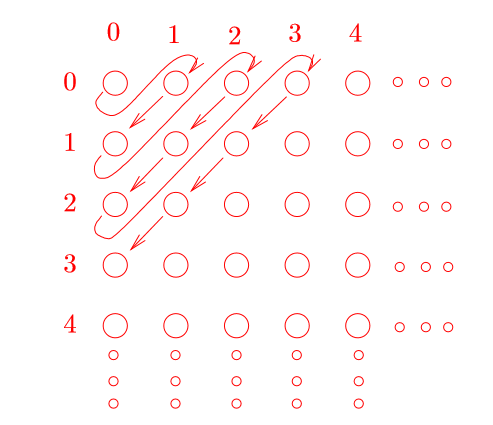
\includegraphics[width=8cm]
		{maths/n2map}}
	\caption{\label{fig:qcount} N and N$^2$}
\end{figure}

\subsection{Relations}
A relation between two sets is a collection of ordered pairs containing one object from each set. If $x \in A$ $y \in B$, then the objects are said to be related if the ordered pair $\left(x,y \right) \in A \times B$ is in the relation.
\paragraph{Relation} Relations are not anything new to us. We have used them in Databases, as SQL is a language focused on relations. Mathematical relations follow the same principle as general relations, but there's some terms we need to speak about.
\paragraph{Reflexivity} We call a binary relation $R \subseteq A \times A$ \textbf{reflexive} if it contains all pairs (x,x) for an element x of A. Let's think of this in a node based graph, where the tuple (a,b) is the connection between a and b. A reflexive set would have all possible tuples where a=b. For example, in the set $A = \left\lbrace a, b, c\right\rbrace$, then it is reflexive if the relations (a,a), (b,b) and (c,c) $\in R$.
If our relation isn't reflexive and we want to make it reflexive, we apply to it what we call \textbf{reflexive-closure}, which returns the smallest set that contains R and is reflexive.
\begin{figure}[!htb]
\center{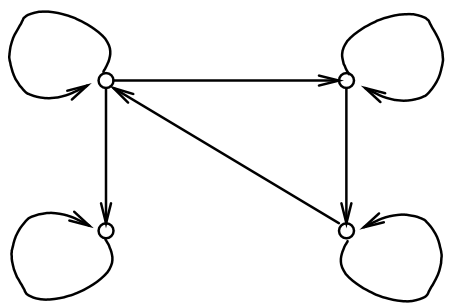
\includegraphics[width=8cm]
	{maths/reflexive}}
\caption{\label{fig:reflexive} Reflexive Nodes}
\end{figure}
\paragraph{Symmetry} We call a binary relation $R \subseteq A \times A$ \textbf{symmetric} if with every pair $\left(x,y \right) \in R$ there is also $\left(y,x \right) \in R$. In the example of path notes, it would mean for every path from a to b (a,b), we have a path leading the other way from b to a (b,a). As with reflexivity, we also have symmetric closure, which is the smallest set that includes R and is symmetric. A neat way to do this is to define an inverse relation by taking all members of $R$ and flipping (x,y) to (y,x). We can then do the set operation union on $R$ and our inverse set $R^{-1}$ and we get the symmetric closure of R.
\begin{figure}[!htb]
	\center{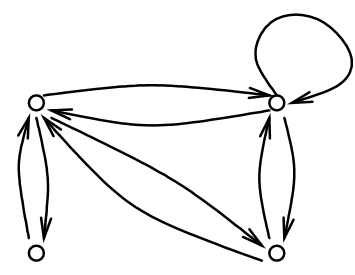
\includegraphics[width=8cm]
		{maths/symmetric}}
	\caption{\label{fig:symmetric} Symmetric Nodes}
\end{figure}
\paragraph{Transitivity} A binary relation $R \subseteq A \times A$ is \textbf{transitive} if whenever $\left(x,y \right) \in R$ and $\left(y,z \right) \in R$ then also $\left(x,z \right) \in R$. Thinking back to the nodes example once more, if we have a path from a to b, and a path from b to c, then there is a direct path from a to c. There is also transitive closure, but it's much more complicated than the previous two.
The trans-closure operation happens more than once, because once new tuples/routes are made, we will have new transitive connections. This operation can repeat forever. It is actually impossible to define transitive closure with the usual means of first order logic. Languages like SQL that are based on first-order logic also don't define transitive closure. Nonetheless, for small enough sets, it should be simple to do by hand.

\paragraph{Types of Relations} We have two packages or properties that we covered in the course. There are \textbf{order relations} and \textbf{equivalence relations}.
\begin{enumerate}
	\item Order Relation: a relation that is reflexive, anti-symmetric and transitive.
	\item Equivalence Relation: a relation that is reflexive, symmetric and transitive.
\end{enumerate}
As we see here, the only difference the two is that one is symmetric, the other is anti-symmetric. Equivalence relations give rise to the concept of classes for items that are loosely equal. For example, the set of rational numbers can give way to some equivalence relations such as (6,10) and (2,3). They both represent the same number and are therefore deemed to be the same class.

\section{Functions}
Expanding from Set Theory, this section deals with Functions and our new understanding of them.
\subsection{Function Definition} For a binary relation $R \subseteq A \times A$ to qualify as a function, two conditions must be met.
\begin{enumerate}
	\item Definedness: For EVERY $a \in A$ there must exist a pair (a,b).
	\item Single Valuedness: For ALL $a \in A$, there is ONLY ONE $b \in B$ such that (a,b) belongs to R.
\end{enumerate}
Relations that satisfy these conditions are called functional relations. Lets clear up some definitions.
\begin{itemize}
	\item If $R \subseteq A \times B$ then A is the \textbf{Domain}.
	\item B is the \textbf{Co-domain}.
	\item The \textbf{Range} is the set of all values in $B$ that are also in $R$. Written as the \textbf{image} of $f$.
\end{itemize}

\paragraph{Properties of Functions} We have three special properties that can apply to a function. 
\begin{enumerate}
	\item Injectivity: A function that will give a different output for each input is injective. Meaning that each element that is in $B$ and in a tuple in $R$, it only appears once.
	\item Surjectivity: A function whose range and co-domain are equal.
	\item Bijectivity: A function that is both injective and surjective is referred to as bijective.
\end{enumerate}

\subsection{Structural Induction}
\paragraph{Defining Syntax} So far, we have created subsets and relations by selection, the thing with the first order logic. This has worked fine for us so far, but problems arise when we want to do stuff like define syntax, or grammar of sorts. For example, the famous set of well balanced brackets. How can we define a set of all strings containing properly nested brackets? We need to define it inductively, using a set of rules.
\begin{enumerate}
	\item The string "[]" $\in A$
	\item If $s \in A$, then "[s]" $\in A$
	\item If $s$ and $t$ are strings that belong to $B$, then $st \in A$
\end{enumerate}
We can use these rules to generate a string like "[][[]]" in steps. We start with Rule 1, and apply rule 2 to it, then apply rule 3 to it with t = "[]", and we have confirmed "[] [[]]" is in the set. This is what we call an inductive function. The base rule, in this case Rule 1, is referred to as the \textbf{base case}. The other rules are referred to as the \textbf{inductive steps}.

\subsection{Structural Induction} To prove properties of an inductive function, we use a process called structural induction. In structural induction, you first assume it works for the base case, and then prove it for each step. This is best with an example. Show that $11^n - 6$ is always divisible by 5 for all n.
\begin{itemize}
	\item Base Case: n = 0
	\item Inductive Hypothesis: Assume $11^n - 6$ is divisible by 5.
	\item Inductive Step: \[ 
	\begin{split}
	11^{n+1} - 6 &= 11^n \times 11 - 6 \\
	&=11^n \times 11 - 66 + 60 \\
	&=11^n \times 11 - (6 \times 11) + 60 \\
	&=11(11^n \times 11 - 6) + 60 \\
	\end{split}\]
\end{itemize}
There are now two terms we need to test for divisibility by 5; $60$ and $11^n - 6$. The first one is obvious. With our hypothesis, we know the second one has to be divisible. Therefore, the inductive rule is valid, and we have proved out induction function.
\section{Probability}
Continuing from Year 1 AI, probability.
\subsection{Definitions}
\begin{itemize}
	\item Sample Space: The range of values of a random variable.
	\item Event: Subset of the sample space; the set of all possible events is the powerset of the sample space. 
	\item Elementary Event: An event with a single outcome.
	\item Probability: A number in the interval [0, 1] that defines the likelihood of an event within a sample space.
\end{itemize}
And here are some common equations and definitions with probabilities.
\begin{itemize}
	\item The probability of an event is a real number greater than 0.
	\item The probably of the sample space is 1.
	\item If $A$ and $B$ are disjoing events, then their union is equivalent to their sum. $p(E \cup F) = p(E) + p(F)$
	\item The complement of the event $A$ is equal to $p(\bar{A} = 1 - p(E))$.
	\item The union of possibly overlapping is different. $p(A \cup B) = p(A) + p(B) - P(A \cap B)$
	\item Independent Experiments: The outcome of the second experiment has nothing to do with the first. $p(A\times B) = p(A) \times p(B)$
	\item Total Correlation: The outcome of the second experiment is determined fully by the outcome of the first, usually determined by a function $f: S \rightarrow T$, the probability. $p(A\times B) = p(A \cap f^{-1}[B])$
	\item Partly Dependent: Much like sampling experiments (4 balls in a bag, 2 black, 2 white, what is the probability the 2nd is white if the first is black?) Best to use decision trees here.
\end{itemize}
\paragraph{Conditional Probability} The conditional probability that $B$ happens given $A$ is written in the form \[p(B|A) = \frac{p(A \cap B)}{p(A)}\]. From this equation, and the fact $p(A \cap B) == p(B \cap A)$, we can derive a formula known as Bayes' Theorem. \[ p(A|B) =\frac{p(A)^*p(B|A)}{p(B)} \] Read as "the probability A occurs given B is true". This formula can also be rewritten as \[ p(A|B) =\frac{p(A)^*p(B|A)}{p(A)^*p(B|A) + p(\bar{A})^*p(B|\bar{A})}\]
\subsection{Discrete Random Variables} 
\paragraph{Random Variables}There is only so much we can do with general sample spaces. So what mathematicians did to make everyone's life harder and more interesting is to map the members of a sample space to real numbers, $\mathbb{R}$. For example, the outcome of ten coin flips has the sample space of 1024 sequences. What we can do instead is point out the number of "heads" in sequence, so the range of the random variable reduces to just 10 members. With numbers now assigned for our events and outcomes, we can start talking about expected values.
\paragraph{Expected Value} The expected value for a random variable $X$ with at most countably many values is the weighted average of all values that X can take: \[ EV(X) = \sum_{i}x_i \times p(x_i) \] For example, a fair 6-sided die would have an expected value of 3.5 ($\frac{1}{6} \times \sum_i^6 i$).
\paragraph{Standard Deviation} It would also be useful to know how much our expected value differs, a sort of range it is expected to be in, because something like 3.5 is not exactly possible from a die. We do this using standard deviation. After calculating EV(X), we can plug it into the variance equation. \[Var(X) = \sum_{i} (x_i - E(X))^2 \times p(x_i)\] and from the variance, we simply take its positive square root to obtain standard deviation. \[SD(X) = \sqrt{Var(X)}\]
\paragraph{Some ol' Classics} Here are some common discrete random variables with some equations.
\begin{itemize}
	\item Bernoulli: Based on the random process wit two outcomes, a and b. $p(a) = q$ and $p(b) = 1 - q$.
	\item Binomial: This is based on using $n$ independent copies of the process and associates each with $2^n$ many outcomes the number of times the outcome $a$ occurred. The probability of the random variable is then $p(X) = (n i) \times p^iq^{n-i}$
	\item Geometric: This is Bernoulli until we obtain an outcome of a, and not just one probability. $p(X) = q^{i-1}p$
	\item Poisson: The outcomes are the natural numbers $\mathbb{N}$ where the probability of each number i is \[ p(X) = \frac{\lambda^i}{i!} \times e^{-\lambda}\] where lambda is a parameter that can be chosen according to the situation we are modeling. $\lambda$ is also the expected value and variance, so $SD(X) = \sqrt{\lambda}$.
\end{itemize}
\subsection{Continuous Random Variables}
\paragraph{Normal Distribution} Continuous random variables are random variables whose range contains no negative numbers and for which the integral from negative infinite to infinite is equal to 1. Given a random variable, it's probability/outcome is determined by an integral in the function; this is referred to as a density function. One of the most common continuous random variables is the normal distribution, the "bell curve" we all know and love. Normal distributions are actually determined by two factors, the expected value $\mu$ and the standard deviation $\sigma$ as $N(\mu, \sigma)$: 
\[
\frac{1}{\sqrt{2\pi}}\times \frac{1}{\sigma} \times e^{-\frac{(x-\mu)^2}{2\sigma^2}}\] 
For which the standard normal distribution, or Gaussian Distribution, is $N(0,1)$. To find expected value, we do an infinite integral of $x f(x) dx$, and similar for variance, where it is the infinite integral of $(x - EV(X))^2f(x)dx$, and standard deviation is not any different.
\paragraph{Central Limit Theorem} 
\section{Equations}
Appending-like area to store all equations that will likely be used in the exam.
